\documentclass[a4paper,oneside,11pt]{article}
\usepackage{graphicx}
\usepackage{ tipa }
\usepackage{hyperref}
\usepackage{titling}
\usepackage{blindtext}
\usepackage{enumitem}
\usepackage{eurosym}
\usepackage{float}
\usepackage{listings}
\usepackage{tabularx}
\usepackage{caption}
\usepackage{pdflscape}
%\captionsetup[figure]{labelformat=empty}


\title{Design Document}
\author{Veljko Tatalović, Nikola Dimić, Edin Žiga}
\date{\today}
\begin{document}
    \begin{titlingpage} 
        \begin{center}
            
\includegraphics[height=5cm]{./RASD-Latex/assets/Logo_Politecnico_Milano.png}\\
            \vspace{4cm}
            \begin{huge} 
                \textbf{\thetitle} \\
            \end{huge}
            \vspace{0.3cm}
            \begin{Large}
                \textit{Students \& Companies} \\
                \vspace{0.3cm}
                \textit{\today}
            \end{Large}
        \end{center}

            \vspace{4cm}
             \begin{large}
            \textbf{Authors:}
            \begin{itemize}
                \item Dimić Nikola
                \item Tatalović Veljko 
                \item Žiga Edin
            \end{itemize}
        \end{large}
    \end{titlingpage}
    \newpage
    \tableofcontents
    \newpage
        
    \section{Introduction}
        \subsection{Purpose}
            This is some text
        \subsection{Scope}
            This is some text
        \subsection{Definitions, Acronyms, Abbreviations}
            \renewcommand{\arraystretch}{1.5}
\subsubsection{Definitions}

\begin{itemize}
    %\item \textbf{Student}: A user of the platform who seeks internship opportunities. Students can upload their CVs, apply for internships, participate in selection processes, file complaints, and provide feedback about completed internships.
    %\item \textbf{Company}: A user of the platform that creates internship advertisements. Companies manage the selection process, evaluate student applications, and provide feedback on the students and the internship experience.
    %\item \textbf{University}: A user of the platform responsible for handling complaints filed by students and monitoring internships to ensure compliance with academic and ethical standards.
    %\item \textbf{Internship}: A professional opportunity created by a company, described with specific details such as required skills, project descriptions, benefits, and the selection process.
    %\item \textbf{Application}: Represents a student's expression of interest in an internship. Each application links a student to a specific internship and includes a status such as Pending, Accepted, or Rejected.
    \item \textbf{Complaint}: A formal request filed by a student to address issues or disputes related to an internship. Complaints are handled and resolved by universities.
    \item \textbf{Feedback}: Insights provided by students or companies about the internship experience. Feedback contributes to platform analytics and recommendations.
    %\item \textbf{CV (Curriculum Vitae)}: A document uploaded by students that outlines their skills, educational background, and work experience. CVs are used by companies to evaluate student applications.
    \item \textbf{Status}: The state of an internship, which can be one of the following: 
        \begin{itemize}
            \item Active: Open for applications and participation.
            \item Closed: Completed or no longer accepting applications.
            \item Draft: In preparation and not visible to students.
        \end{itemize}
    %\item \textbf{Application Status}: The state of a student's application for an internship. Possible statuses include:
        %\begin{itemize}
            %\item Pending: Awaiting review by the company.
            %\item Accepted: Approved by the company.
            %\item Rejected: Not approved by the company.
        %\end{itemize}
    \item \textbf{Recommendation System}: A feature of the platform that suggests internships to students based on their uploaded CVs, skills, and preferences.
    %\item \textbf{Selection Process}: The procedure defined by companies for evaluating student applications. This may include questionnaires, interviews, and multi-round assessments.
    \item \textbf{Complaint Resolution}: The process carried out by universities to address and resolve issues raised by students regarding internships.
    %\item \textbf{Internship Monitoring}: The process by which universities oversee the progress and compliance of active internships, ensuring alignment with academic and ethical standards.

\end{itemize}

\subsubsection{Acronyms}
\begin{itemize}
    \item AI: Artificial Intelligence
    \item API: Application Protocol Interface
    \item AWS: Amazon Web Service
    \item S\&C: Students \& Companies
    \item UI: User Interface
\end{itemize}
\subsubsection{Abbreviations}
\begin{itemize}
    \item FR*: Functional Requirement
    \item UC*: Use Case
    \item HR*: Human Resources
\end{itemize}

        \subsection{Revision history}
            \textbf{v1.0} - 25/12/2024 - Initial release \\
\textbf{v1.1} - 28/12/2024 - Finished section 1 \\
\textbf{v1.2} - 02/01/2025 - Draft Section 2, Section 3 \\
\textbf{v1.3} - 4/01/2024 - Finalized diagrams for section section 2 \& 3, section 4 and 5 draft \\
\textbf{v1.4} - 7/01/2024 - Finalized all sections, spell check \\


        \subsection{Reference documents}
            The document is based on the following materials:

\begin{itemize}
    \item The specification of the \textit{RASD} and \textit{DD} assignment of the
    \textit{Software Engineering II} course a.a. 2024/25
    \item Slides of the course on WeBeep
    \item  Larman, C. (2002). Applying UML and patterns: An introduction to
object-oriented analysis and design and the Unified Process. Prentice
Hall PTR.
\end{itemize}




        \subsection{Document structure}
            \renewcommand{\arraystretch}{1.6}
This DD document consists of the following parts:
\begin{enumerate}
    \item \textbf{Introduction}: A brief description of the project that is focused on the purpose, the goals that are aimed to be achieved, and the scope that is covered with its development.
    \item \textbf{Architectural Design}: Shows how Students\&Companies is built on a three-tier setup hosted on AWS, using containerization for easy scaling. It highlights key back-end managers for core functionalities and illustrates how the system can run multiple instances across different servers as needed.
    \item \textbf{User Interface Design }: Presents possible layouts of the user interface for the mobile and
desktop applications.
    \item \textbf{Requirements Traceability}: Explains how the requirements defined in the RASD map the design components explained in this document.
    \item \textbf{ Implementation, Integration and Test Plan}: Detailed explanation of how the platform described in the previous sections will be developed and tested.
    \item \textbf{ Effort Spent}: the references to any documents and software used to create this document.
\end{enumerate}
        
    \newpage
    \section{Architectural Design}
        \subsection{Overview}
            As the S\&C platform will be entirely hosted using Amazon Web Services (AWS), by its design it will utilize the three layer architecture, consisting of the presentation layer for the user interface and interaction, the application layer for data processing, and lastly, the database layer where all application data will be stored. The choice for AWS and subsequently this style came from the ease of deployment, as AWS provides a ready made solution for this type of application.

\begin{figure}[h]
    \centering
    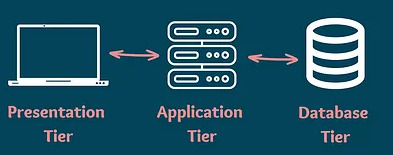
\includegraphics[width=0.75\linewidth]{DD-Latex//assets/Three tier.jpg}
    \caption{Three tier architecture \cite{MToC_2023}}
    \label{fig:enter-label}
\end{figure}

\subsubsection{Distributed view}

        \subsection{Component view}
            \begin{figure}[h]
    \centering
    \includegraphics[width=1\linewidth]{DD}
    \caption{Three tier architecture \cite{MToC_2023}}
    \label{fig:enter-label}
\end{figure}
        \subsection{Deployment view}
            This is some text
        \subsection{Runtime view}
            The following section presents the runtime view diagrams for each use case outlined in the RASD v1 document accompanying this report. It covers 17 use cases and illustrates the interactions between the system's components. It is important to note that the API interface artifact has been excluded from the diagrams to avoid unnecessary clutter, as its inclusion offers little to no benefit to the communication process between components. For the sake of simplicity, this section assumes that the API is integrated as part of the AWS Server component.
\newpage
\begin{enumerate}[label={[UC\arabic*]}]
    \item Student and University User Registration
    \begin{figure}[h]
        \centering
        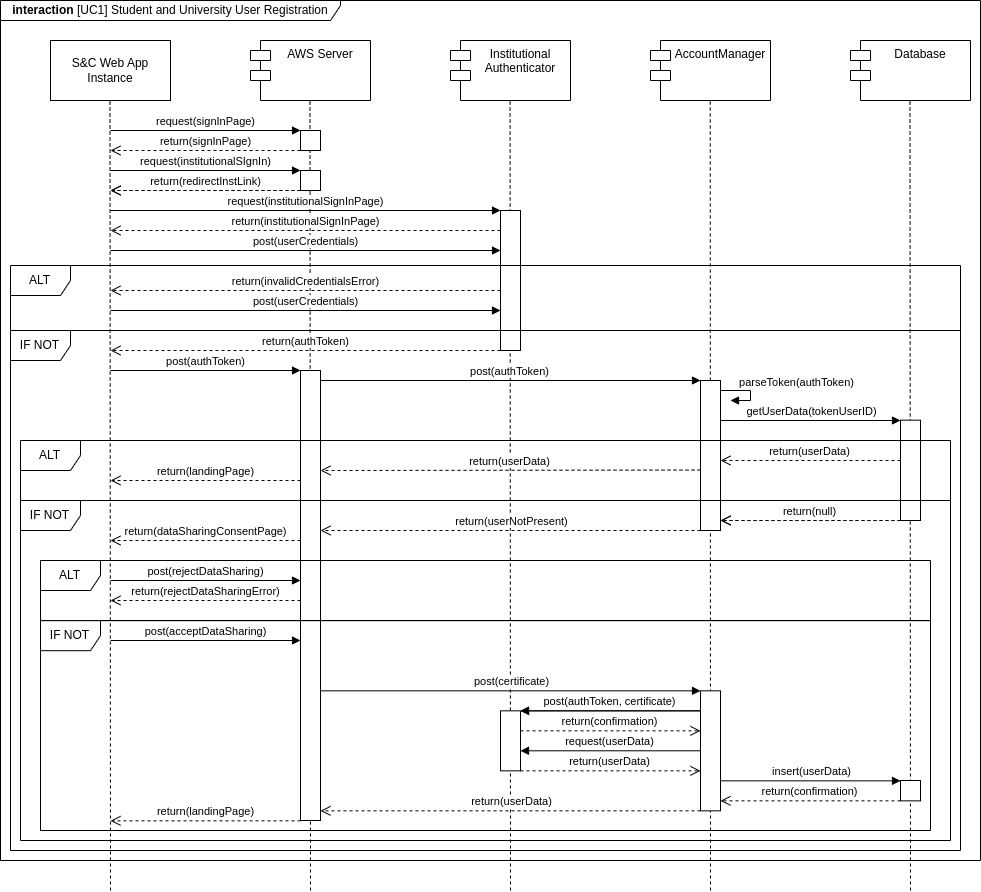
\includegraphics[width=1\linewidth]{DD-Latex//assets//Runtime View Diagrams/UC1.jpg}
        \caption{UC1 - Runtime View Diagram}
        \label{fig:UC1}
    \end{figure}
    
    The diagram in Figure 5 illustrates the interactions between system components during the Student and University user registration process. As noted, the system supports the use of an external authenticator (such as Microsoft 365), which provides the data required to set up a user's profile. The diagram shows the data transfer and storage in the platform's database at the final step, while the preceding elements depict the communication and exchange of the authentication token between various system components.
    \newpage
    \item Student and University User Login
    \begin{figure}[h]
        \centering
        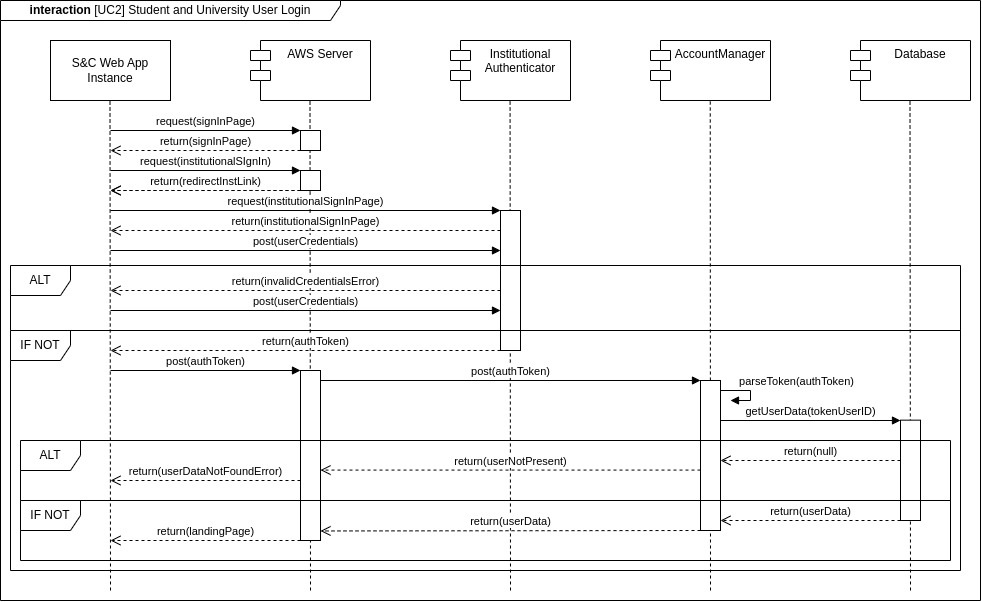
\includegraphics[width=1\linewidth]{DD-Latex//assets//Runtime View Diagrams/UC2.jpg}
        \caption{UC2 - Student and University User Registration}
        \label{fig:UC2}
    \end{figure}

    The second diagram can be considered a derivative of the first, as the communication process closely resembles that of the registration process. It should be noted that the final alternative flow depicted in this diagram actually marks the beginning of the registration process. If a user attempts to authenticate with an account that is not registered with the service, the system will automatically initiate the sign-in process.
    \newpage
    
    \item Register Company User
    \begin{figure}[h]
        \centering
        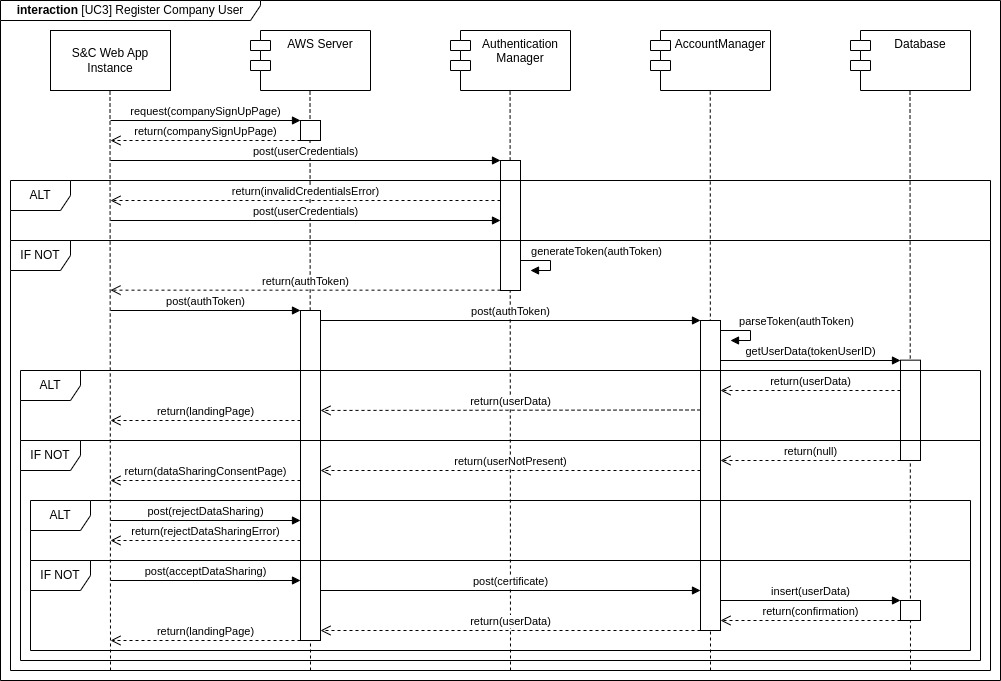
\includegraphics[width=1\linewidth]{DD-Latex//assets//Runtime View Diagrams/UC3.jpg}
        \caption{UC3 - Register Company User}
        \label{fig:UC3}
    \end{figure}
    
    The company user registration process is very similar to the student and university user registration, except that companies do not have access to external authentication services, unlike students and universities. The communication process remains largely the same throughout.

    \newpage
    \item Login Company User
    \begin{figure}[h]
        \centering
        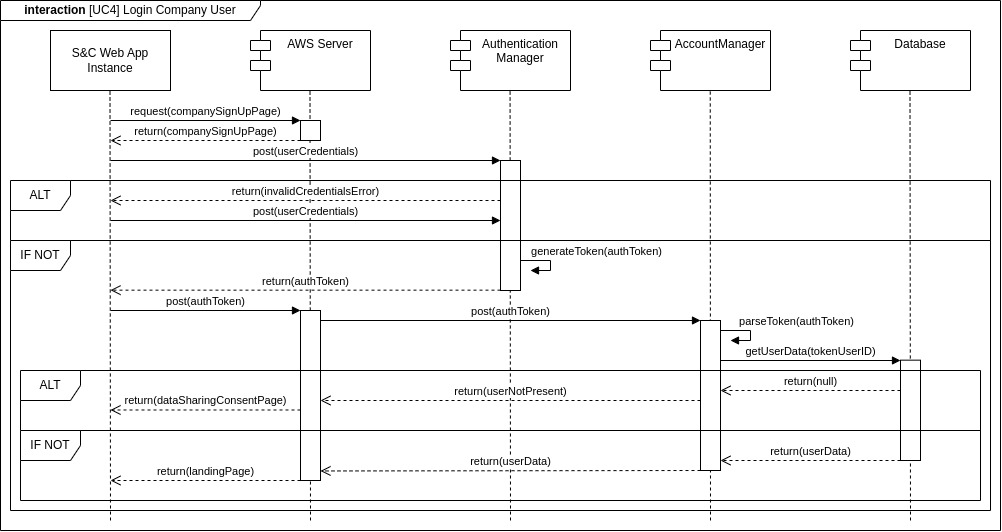
\includegraphics[width=1\linewidth]{DD-Latex//assets//Runtime View Diagrams/UC4.jpg}
        \caption{UC4 - Login Company User}
        \label{fig:UC4}
    \end{figure}
    
    As before, the login diagram is essentially a variation of the sign-up diagram, as the communication remains largely similar between the two processes. It should be noted that the final alternative flow presented leads to the option of signing up a new company user.
    
    \item Edit profile
    \begin{figure}[h]
        \centering
        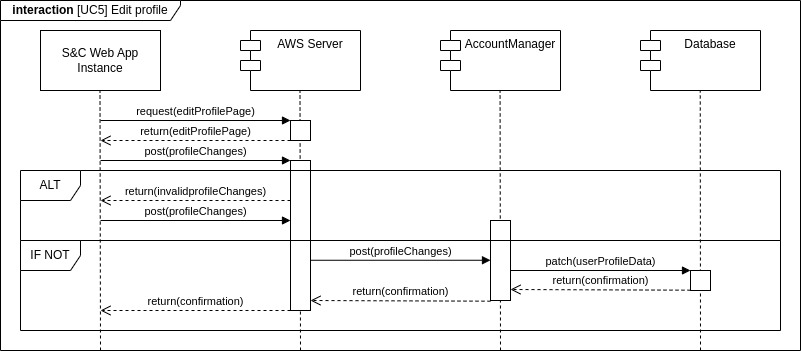
\includegraphics[width=1\linewidth]{DD-Latex//assets//Runtime View Diagrams/UC5.jpg}
        \caption{UC5 - Edit profile}
        \label{fig:UC5}
    \end{figure}

    The edit profile interaction assumes that the user is fully authenticated and has accessed the platform's landing page, as outlined in the original use case in the provided RASD v1 document. This explains the absence of the Authentication Manager component. Furthermore, the Account Manager component handles most of the required edits during this interaction.
    
    \item Create and Publish Internship Advertisement
    \begin{figure}[h]
        \centering
        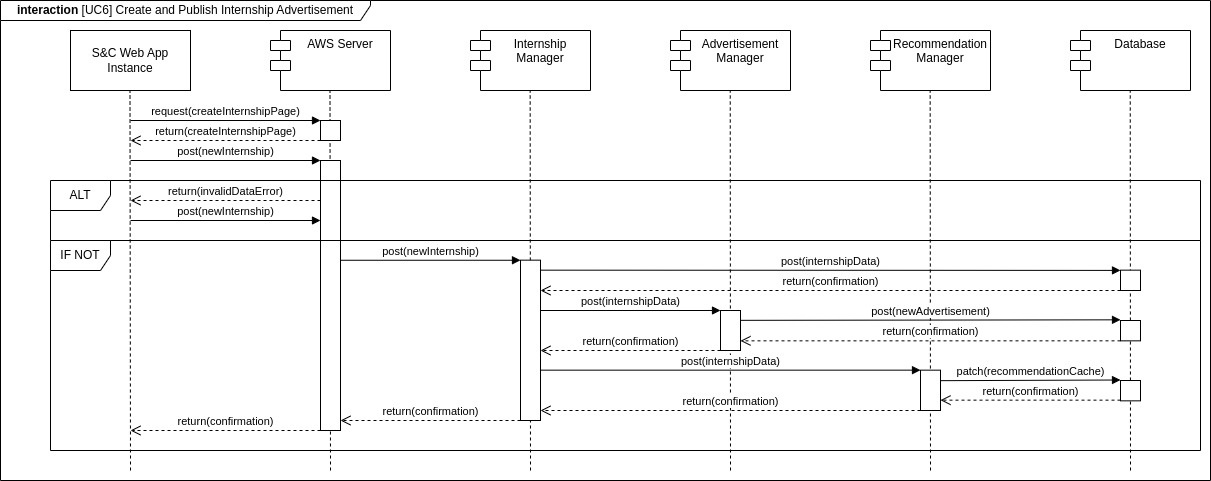
\includegraphics[width=1\linewidth]{DD-Latex//assets//Runtime View Diagrams/UC6.jpg}
        \caption{UC6 - Create and Publish Internship Advertisement}
        \label{fig:UC6}
    \end{figure}

    The sixth use case, which involves creating and publishing a new internship advertisement, includes some complex interactions to achieve the desired functionality. These interactions primarily occur between the Internship Manager, the Advertisement Manager, and the Recommendation Manager, as the latter two depend on the Internship Manager's functionality. The Internship Manager creates the internship in the database and then passes the relevant internship data to enable the creation and publication of the advertisement, as well as to update the recommendations cache.
    
    \item Edit Internship Advertisement
    \begin{figure}[h]
        \centering
        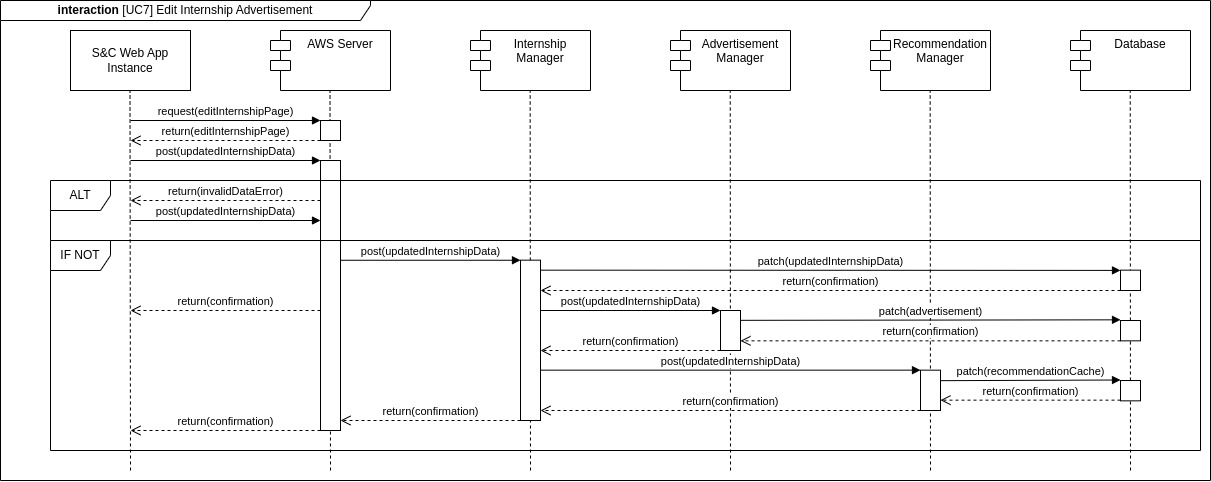
\includegraphics[width=1\linewidth]{DD-Latex//assets//Runtime View Diagrams/UC7.jpg}
        \caption{UC7 - Edit Internship Advertisement}
        \label{fig:UC7}
    \end{figure}

    The interactions required for editing an active internship advertisement are largely similar, if not identical, to those in UC6, with the main difference being the type of operations conducted between certain components (primarily, inserts being replaced with patches).
    
    \item Delete Internship Advertisement
     \begin{figure}[h]
        \centering
        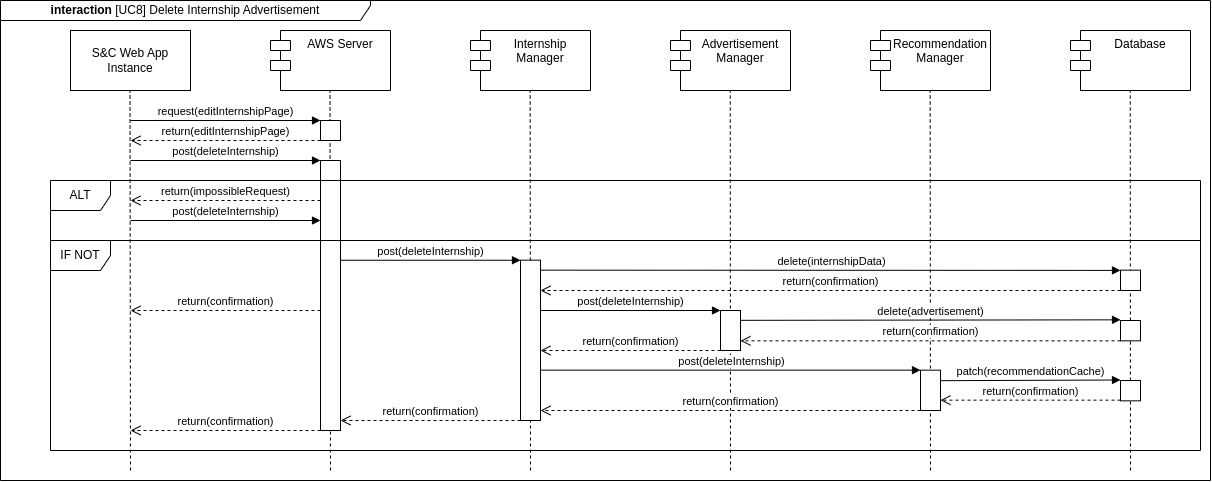
\includegraphics[width=1\linewidth]{DD-Latex//assets//Runtime View Diagrams/UC8.jpg}
        \caption{UC8 - Delete Internship Advertisement}
        \label{fig:UC8}
    \end{figure}

    As with the previous two use cases, the interactions between the components remain largely the same, with minor changes to the types of operations (specifically, inserts/patches being replaced by delete operations).
    
    \item View Recommendations \& Offerings, Apply for Internship
    \begin{figure}[h]
        \centering
        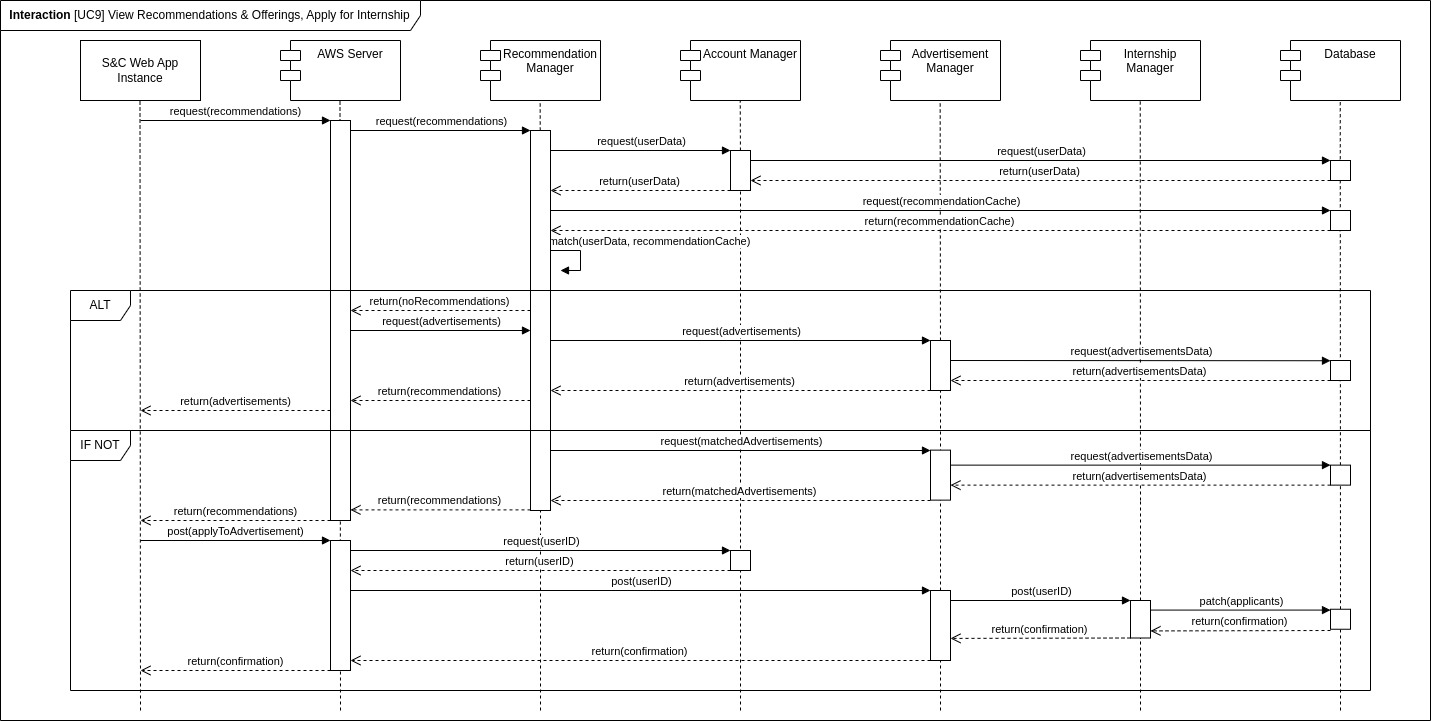
\includegraphics[width=1\linewidth]{DD-Latex//assets//Runtime View Diagrams/UC9.jpg}
        \caption{UC9 - View Recommendations \& Offerings, Apply for Internship}
        \label{fig:UC9}
    \end{figure}

    The UC9 Runtime View diagram represents one of the more complex diagrams in this section. For simplification, it can be divided into two stages: the first stage involves fetching or generating relevant recommendations for a single user, while the second stage covers the application process for a single internship advertisement.

    In the first stage, the Recommendations Manager gathers data based on the logged-in user's profile and retrieves its stored cache of internship advertisements from the database. Once the required data is retrieved, a matching algorithm runs to provide the user with advertisements relevant to their profile. An alternative flow exists where, if no match is found, the system returns a randomized set of advertisements.

    The second stage handles the application process, which involves much simpler inter-component communication compared to the first stage, as shown in the diagram.
    
    \item Change candidate status (increment or reject)
    \begin{figure}[h]
        \centering
        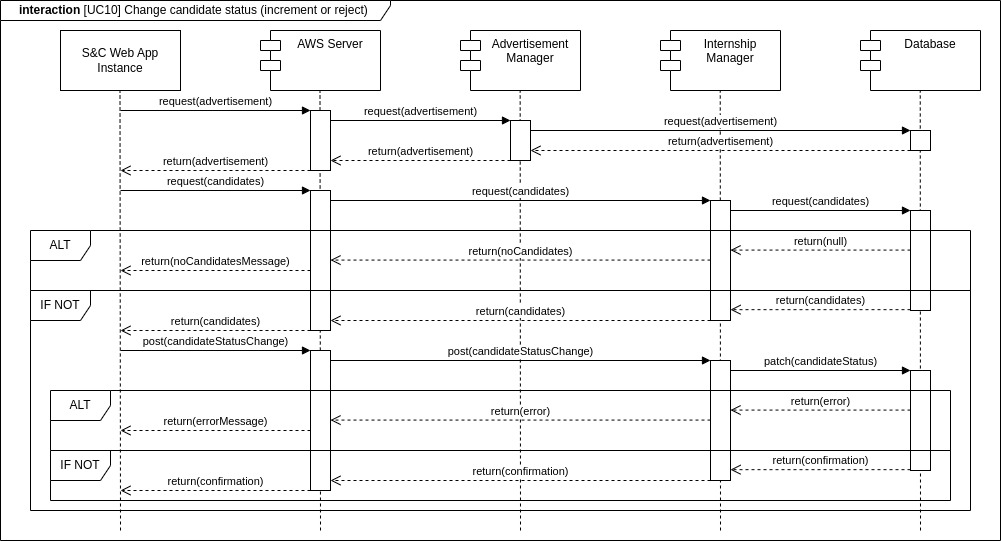
\includegraphics[width=1\linewidth]{DD-Latex//assets//Runtime View Diagrams/UC10.jpg}
        \caption{UC10 - Change candidate status (increment or reject)}
        \label{fig:UC10}
    \end{figure}

    UC10 illustrates the communication required to change a candidate's status. It begins by fetching all advertisements relevant to the user, and once one is selected, it retrieves all the candidates for that internship. An alternative flow exists for the scenario where no candidates have applied for the specific internship. Otherwise, the sequence continues by issuing a patch to the database for the selected candidate.

    \newpage
    \item Send Prompt to Candidate (questionnaire or interview invitation)

     \begin{figure}[h]
        \centering
        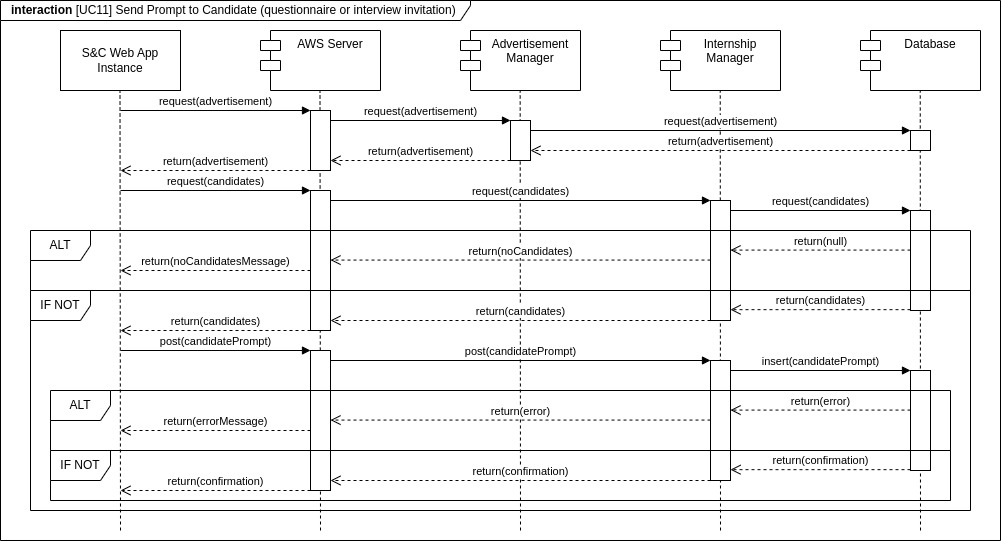
\includegraphics[width=1\linewidth]{DD-Latex//assets//Runtime View Diagrams/UC11.jpg}
        \caption{UC11 - Send Prompt to Candidate (questionnaire or interview invitation)}
        \label{fig:UC11}
    \end{figure}

    UC11 follows many of the same sequences presented in UC10, with the main differences lying in the types of communications between the components, such as patches being substituted for inserts.

    \item Reply to invitation

    \begin{figure}[h]
        \centering
        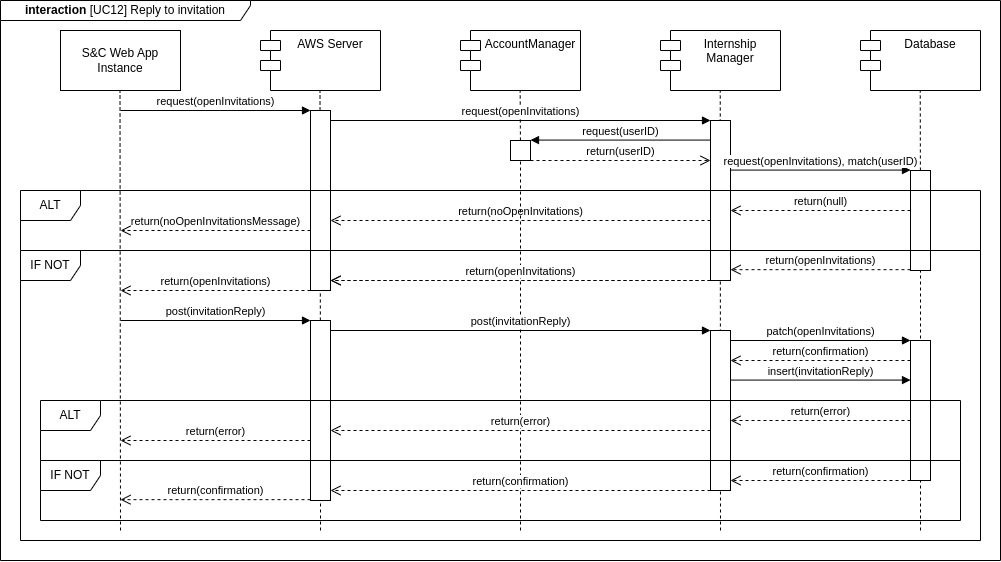
\includegraphics[width=0.90\linewidth]{DD-Latex//assets//Runtime View Diagrams/UC12.jpg}
        \caption{UC12 - Reply to invitation}
        \label{fig:UC12}
    \end{figure}

    Like UC11, the required interaction for UC12 is largely similar, but it contains a subtle difference, as two distinct database edits are required to complete it. First, a patch operation is performed to close the open invitation, followed by an insert operation to add the reply to the database.
    
    \item Initiate Internship
    \begin{figure}[h]
        \centering
        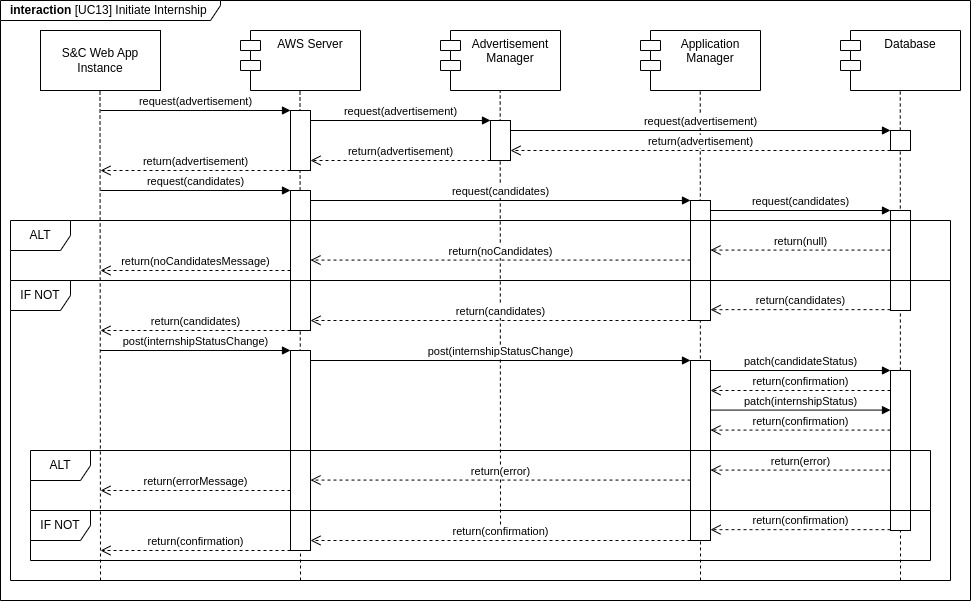
\includegraphics[width=1\linewidth]{DD-Latex//assets//Runtime View Diagrams/UC13.jpg}
        \caption{UC13 - Initiate Internship}
        \label{fig:UC13}
    \end{figure}

    UC13's communication process can be viewed as a mix of several presented use cases, with a degree of overlap between them. Ultimately, it comes down to having candidates who are eligible for the start of an internship, as well as two database edits required to initiate it.
    
    \item Submit Complaint

    \begin{figure}[h]
        \centering
        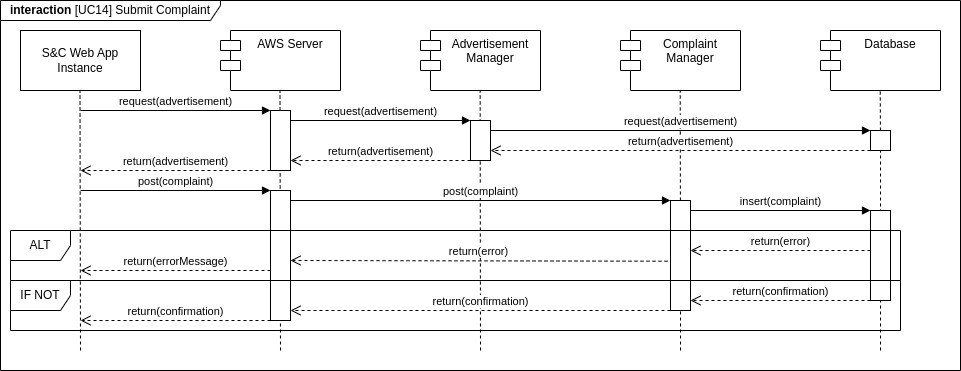
\includegraphics[width=1\linewidth]{DD-Latex//assets//Runtime View Diagrams/UC14.jpg}
        \caption{UC14 - Submit Complaint}
        \label{fig:UC14}
    \end{figure}

    The submit complaint runtime view is one of the simpler views in this document, as the interactions required among the components for its functionality are minimal. As shown in the diagram, the main actor is the complaint manager, who processes the complaint.
    
    \item Resolve complaint

    \begin{figure}[h]
        \centering
        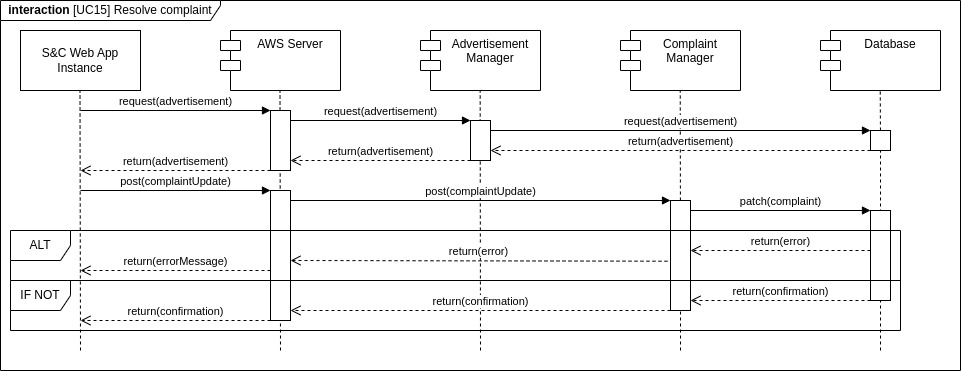
\includegraphics[width=1\linewidth]{DD-Latex//assets//Runtime View Diagrams/UC15.jpg}
        \caption{UC15 - Resolve complaint}
        \label{fig:UC15}
    \end{figure}

    As with many other use cases, UC15 is a simple variation of UC14, where the required operations are merely adjusted for the specific use case.
    
    \item Submit feedback

    \begin{figure}[h]
        \centering
        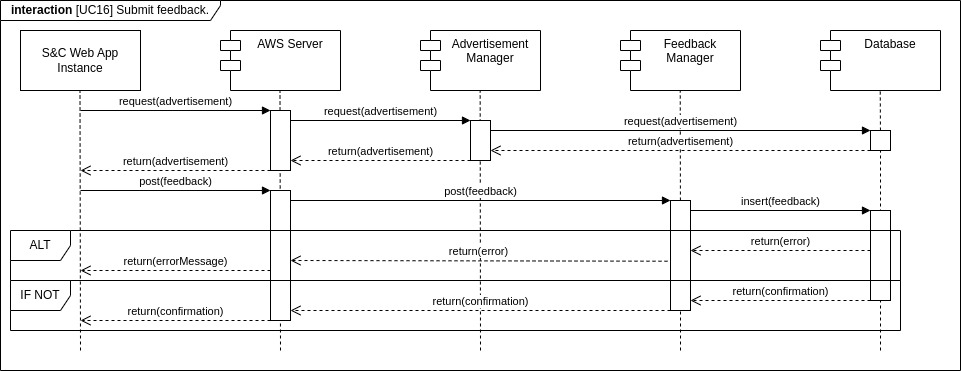
\includegraphics[width=1\linewidth]{DD-Latex//assets//Runtime View Diagrams/UC16.jpg}
        \caption{UC16 - Submit feedback}
        \label{fig:UC16}
    \end{figure}

    For the submission of feedback, there is a requirement that an internship be finished (either by its natural course or by early termination). Afterward, users may submit feedback, which is handled through the feedback manager, as shown in the diagram.
    \newpage
    
    \item View feedback

    \begin{figure}[h]
        \centering
        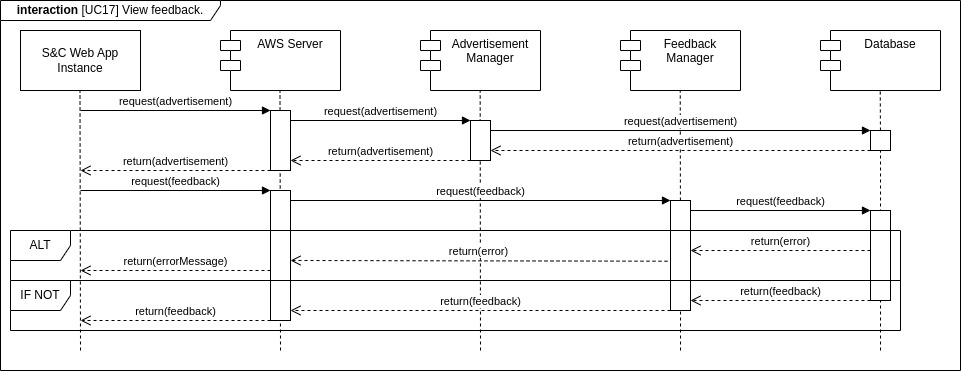
\includegraphics[width=1\linewidth]{DD-Latex//assets//Runtime View Diagrams/UC17.jpg}
        \caption{UC17 - View feedback}
        \label{fig:UC17}
    \end{figure}

    Lastly, the view feedback interaction is a simple variation of UC16, and like many of the previous ones, consists of minor changes in the types of interactions between the components.
\end{enumerate}
        \subsection{Component interfaces}
            \begin{enumerate}
    \item \textbf{AccountManager}
    \begin{enumerate}
        \item getUserData(tokenUserID)
        \item insert(userData)
        \item parseToken(authToken)
        \item post(authToken, certificate)
        \item request(userData)
        \item return(userData)
        \item return(userID)
        \item return(userNotPresent)
    \end{enumerate}
    \item \textbf{AdvertisementManager}
    \begin{enumerate}
        \item delete(advertisement)
        \item patch(advertisement)
        \item post(newAdvertisement)
        \item post(userID)
        \item request(advertisements)
        \item return(confirmation)

    \end{enumerate}
    \item \textbf{AuthenticationManager}
    \begin{enumerate}
        \item generateToken(authToken)
        \item return(authToken)
        \item return(confirmation)
        \item return(invalidCredentialsError)
        \item return(institutionalSignInPage)
        \item return(userData)

    \end{enumerate}
    \item \textbf{AWS Server}
    \begin{enumerate}
        \item post(authToken)
        \item post(certificate)
        \item post(deleteInternship)
        \item post(feedback)
        \item post(internshipStatusChange)
        \item post(invitationReply)
        \item post(newInternship)
        \item post(updatedInternshipData)
        \item request(advertisement)
        \item request(candidates)
        \item request(feedback)
        \item request(openInvitations)
        \item request(recommendations)
        \item request(userID)
        \item return(advertisement)
        \item return(confirmation)
        \item return(dataSharingConsentPage)
        \item return(editProfilePage)
        \item return(impossibleRequest)
        \item return(invalidProfileChanges)
        \item return(landingPage)
        \item return(noOpenInvitations)
        \item return(openInvitations)
        \item return(rejectDataSharingError)
        \item return(signInPage)
        \item return(redirectLink)
        \item return(userData)
        
    \end{enumerate}
    \item \textbf{ComplaintManager}
    \begin{enumerate}
        \item insert(complaint)
        \item patch(complaint)
        \item return(confirmation)
        \item return(error)

    \end{enumerate}
    \item \textbf{Database}
    \begin{enumerate}
        \item return(advertisement)
        \item return(confirmation)
        \item return(error)
        \item return(userData)

    \end{enumerate}
    \item \textbf{FeedbackManager}
    \begin{enumerate}
        \item insert(feedback)
        \item request(feedback)
        \item return(confirmation)
        \item return(error)

    \end{enumerate}
    \item \textbf{InstitutionalAuthenticator}
    \begin{enumerate}
        \item return(authToken)
        \item return(confirmation)
        \item return(institutionalSignInPage)
        \item return(invalidCredentialsError)
        \item return(userData)

    \end{enumerate}
    \item \textbf{InternshipManager}
    \begin{enumerate}
        \item delete(internshipData)
        \item insert(application)
        \item insert(candidatePrompt)
        \item insert(invitationReply)
        \item patch(internshipStatus)
        \item patch(openInvitations)
        \item patch(updatedInternshipData)
        \item post(deleteInternship)
        \item post(internshipData)
        \item request(candidates)
        \item request(openInvitations)
        \item request(userID)
        \item return(error)
        \item return(noCandidates)
        \item return(noOpenInvitations)
        \item return(signInPage)
    \end{enumerate}
    \item \textbf{RecommendationManager}
    \begin{enumerate}
        \item match(userData, recommendationCache)
        \item patch(recommendationCache)
        \item request(advertisements)
        \item request(matchedAdvertisements)
        \item request(recommendationCache)
        \item request(userData)
        \item return(confirmation)
        \item return(recommendations)

    \end{enumerate}
    \item \textbf{S\&C Web App Instance}
    \begin{enumerate}
        \item post(acceptDataSharing)
        \item post(applyToAdvertisement)
        \item post(candidatePrompt)
        \item post(complaint)
        \item post(complaintUpdate)
        \item post(feedback)
        \item post(invitationReply)
        \item post(internshipStatusChange)
        \item post(profileChanges)
        \item post(rejectDataSharing)
        \item post(updatedInternshipData)
        \item request(advertisement)
        \item request(candidates)
        \item request(editProfilePage)
        \item request(feedback)
        \item request(institutionalSignIn)
        \item request(institutionalSignInPage)
        \item request(openInvitations)
        \item request(recommendations)
        \item request(signInPage)
        \item return(landingPage)
        \item return(noOpenInvitations)
        \item return(openInvitations)
    \end{enumerate}
\end{enumerate}

        \subsection{Selected architectural styles and patterns}
            \subsubsection{Three-Tier Architecture}
As mentioned earlier, the platform will be fully implemented using AWS, which is regarded as one of the best examples of the three-tier architecture. More details can be found at the beginning of this section regarding the exact implementation for this specific platform, but in essence,

\subsubsection{Model-View-Controller Pattern}
For an application like this one, utilizing the Model-View-Controller (MVC) pattern is a logical choice. Given the chosen application hosting solution, using this pattern makes development much quicker and easier for all parties involved, while providing many benefits for long-term system evolution.

\subsubsection{Facade Pattern}
As the system will undoubtedly evolve over time with the addition of new features and many other adaptations, it will utilize the Facade pattern to simplify the interaction process as the number of subsystems increases. This makes system changes and evolution easier to manage.
        \subsection{Other design decisions}
            This is some text

    \newpage
    \section{User Interface Design}
        In this chapter, the possible layouts of the user interface for the mobile and desktop applications are presented.
\bigskip
\bigskip

\begin{figure}[ht]
    \centering
    \begin{minipage}[b]{0.45\textwidth}
        \centering
        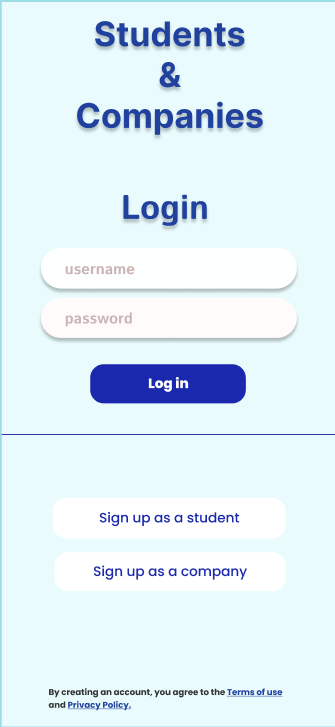
\includegraphics[width=\textwidth]{RASD-Latex/assets/UI images/login_phone.png}
        \caption{Log in form on mobile application}
        \label{fig:image1}
    \end{minipage}
    \hfill
    \begin{minipage}[b]{0.45\textwidth}
        \centering
        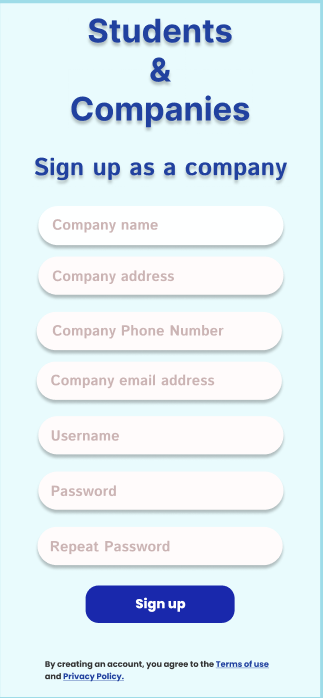
\includegraphics[width=\textwidth]{RASD-Latex/assets/UI images/signup_company_phone.png}
        \caption{Sign up for companies on mobile application}
        \label{fig:image2}
    \end{minipage}
\end{figure}


\begin{figure}[ht]
    \centering
    \begin{minipage}{0.45\textwidth}
        \centering
        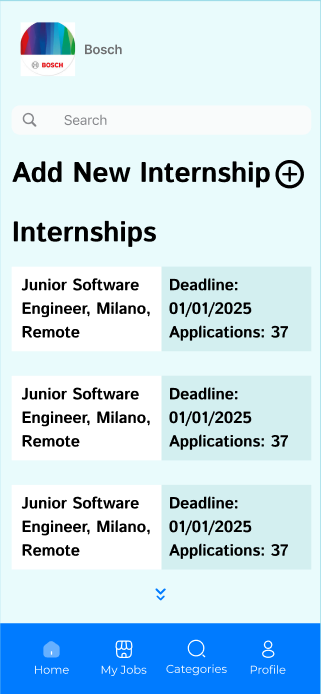
\includegraphics[width=\textwidth]{RASD-Latex/assets/UI images/mainpage_company_phone.png}
        \caption{Main page for companies on mobile application}
        \label{fig:image1}
    \end{minipage}
    \hspace{0.05\textwidth}  % Optional space between the images
    \begin{minipage}{0.45\textwidth}
        \centering
        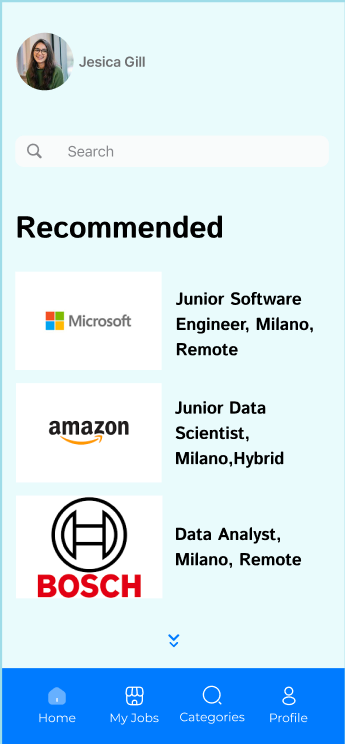
\includegraphics[width=\textwidth]{RASD-Latex/assets/UI images/mainpage_student_phone.png}
        \caption{Main page for students on mobile application}
        \label{fig:image2}
    \end{minipage}
\end{figure}

\clearpage

\begin{figure}[h!]
    \centering
    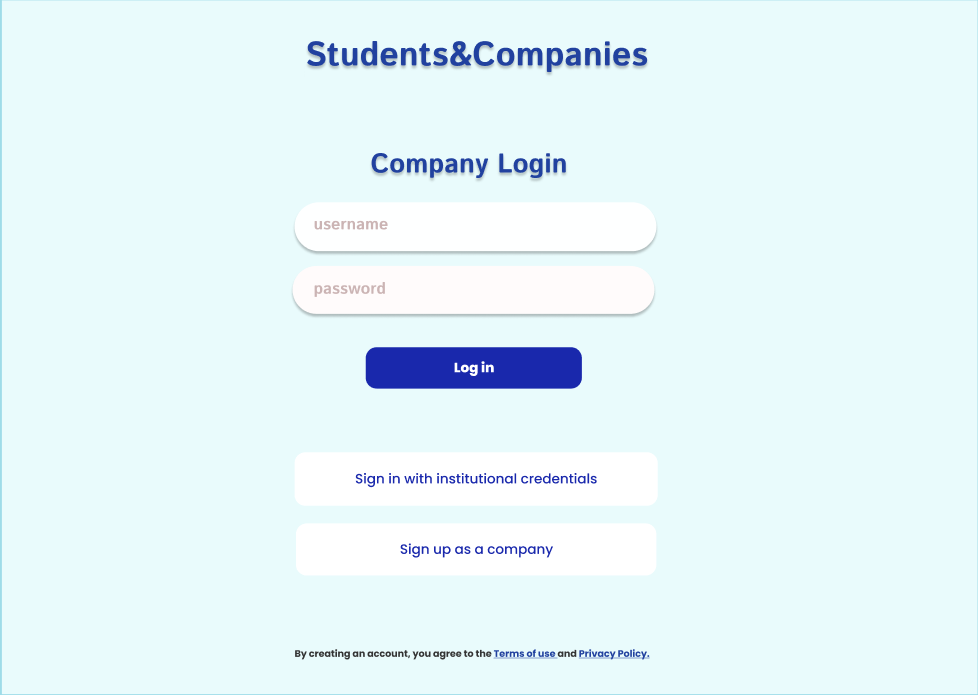
\includegraphics[width=0.8\textwidth]{RASD-Latex/assets/UI images/login_desktop.png}
    \caption{Log in form on desktop application}
    \label{fig:image1}
\end{figure}


\begin{figure}[h!]
    \centering
    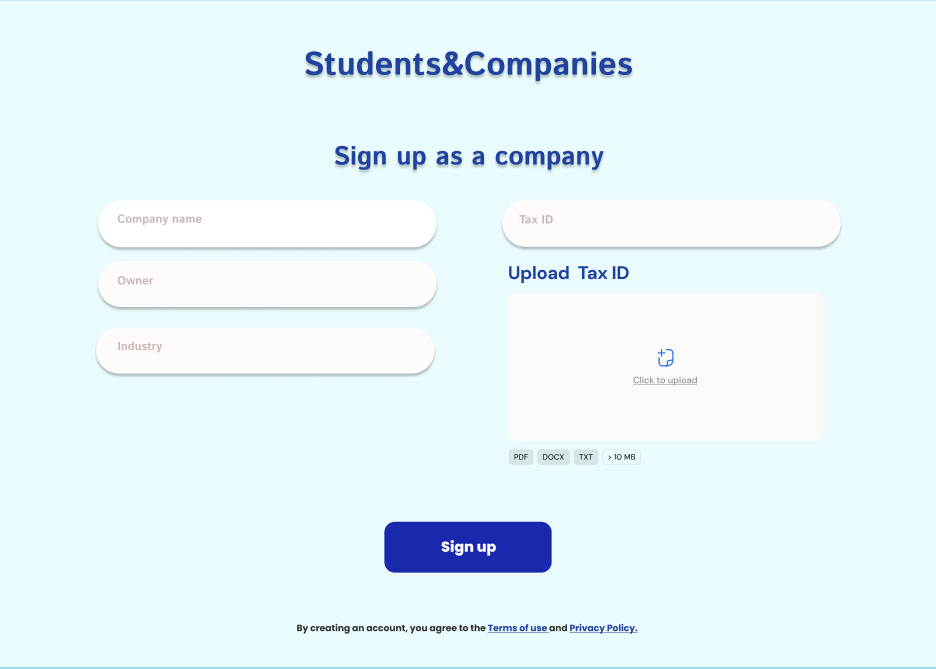
\includegraphics[width=0.8\textwidth]{RASD-Latex/assets/UI images/signup_company_desktop.png}
    \caption{Sign up for companies on desktop application}
    \label{fig:image1}
\end{figure}


\begin{figure}[ht]
    \centering
    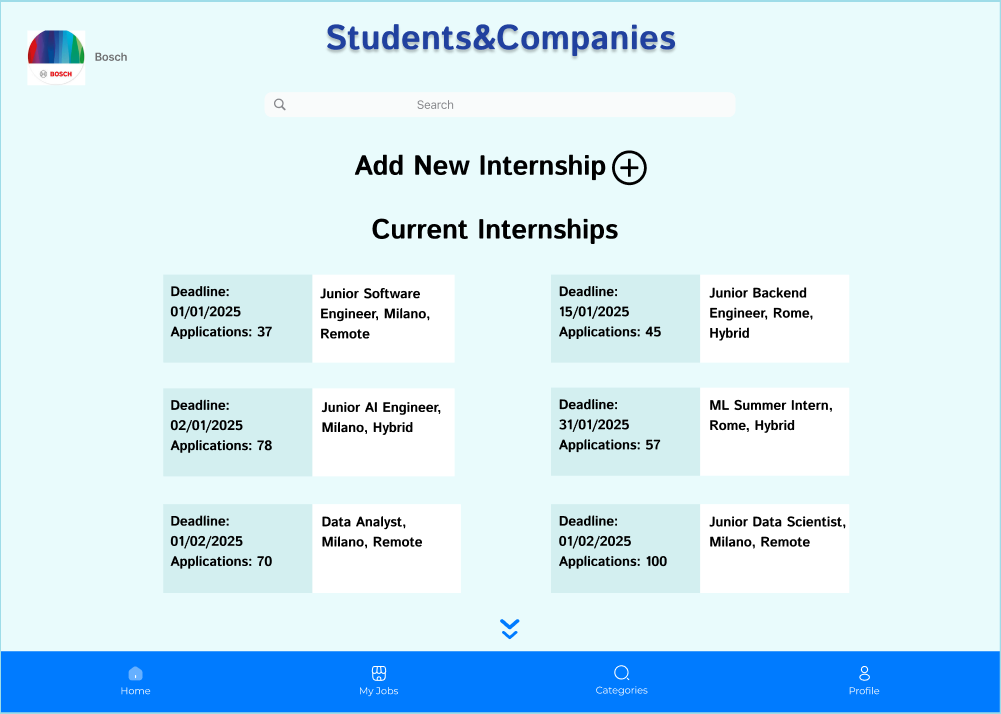
\includegraphics[width=0.8\textwidth]{RASD-Latex/assets/UI images/mainpage_company_desktop.png}
    \caption{Main page for companies on desktop application}
    \label{fig:image1}
\end{figure}


\begin{figure}[ht]
    \centering
    
\includegraphics[width=0.8\textwidth]{RASD-Latex/assets/UI images/mainpage_student_desktop.png}
    \caption{Main page for students on desktop application}
    \label{fig:image2}
\end{figure}

\clearpage

    \newpage
    \section{Requirements Traceability}
        % Define new column types in the preamble
\newcolumntype{C}[1]{>{\centering\arraybackslash}m{#1}}
\newcolumntype{L}[1]{>{\raggedright\arraybackslash}m{#1}}


% Table 1
\begin{table}[ht]
    \centering
    \renewcommand{\arraystretch}{1.5} % Adjust row spacing
    \begin{tabular}{|p{0.3\textwidth}|p{0.65\textwidth}|} % Allow text wrapping
        \hline
        \textbf{Requirements} & 
        \textbf{Registration of Students} \par
        [R1] The system shall allow new student users to register on the platform using their respective institutional accounts. \par
        [R2] After an institutional account has been linked with the platform, the system shall allow student users to log in using their institutional credentials. \par
        [R3] The system shall allow the registration of student users only if they are classified as students within the institutional account they provide. \\
        \hline
        \textbf{Components} & 
        WebApp \par
        API \par
        AuthenticationManager \par
        AccountManager \par
        Database \par
        GitHub \\
        \hline
    \end{tabular}
\end{table}


% Table 2
\begin{table}[h]
    \centering
    \renewcommand{\arraystretch}{1.5} % Adjust row spacing
    \begin{tabular}{|C{0.3\textwidth}|L{0.65\textwidth}|} % Left column centered, right column left-aligned
        \hline
        \textbf{Requirements} &    
         \textbf{Registration of Companies}
         \newline
        [FR4] The system shall allow new company users to register on the platform using a valid email address.
        \newline
        [FR5] After providing an email address, the system shall verify the provided address through a verification email. 
        \newline
        [FR6] After the new company user has verified their email, the system shall generate and deliver a password for the newly created account via the verified email. 
        \newline
        [FR7] The system shall allow the company user to log in using the validated email address and the provided password. 
        \newline
        [FR8] Upon the first login, the system shall require the new user to provide a certificate from the relevant tax authority, including the company name and unique identifier. The system shall also require the full company name and unique identifier to be entered manually in the relevant input fields alongside the certificate. 
        \newline
        [FR9] The system shall retain company user data only at two points: first, after successful email verification, where the provided email address and generated password will be retained as login credentials; and second, after submitting the initial verification information, where all submitted data up to that point shall be retained. 
        \\
        \hline
        \textbf{Components} & WebApp \newline API \newline AuthenticationManager \newline AccountManager \newline Database \newline GitHub \\
        \hline
    \end{tabular}
\end{table}

%Table 3
\begin{table}[h]
    \centering
    \renewcommand{\arraystretch}{1.5} % Adjust row spacing
    \begin{tabular}{|C{0.3\textwidth}|L{0.65\textwidth}|} % Left column centered, right column left-aligned
        \hline
        \textbf{Requirements} & 
        \textbf{Registration of Universities} \par
        [FR10] The system shall allow new university users to register on the plat-
        form using pre-designated institutional accounts allocated for S\&C. \par
        [FR11] After an institutional account has been linked with the platform,
        the system shall allow university users to log in using their institu-
        tional credentials. \par
        [FR12] If the institutional account has not been pre-designated for use on
        S\&C, the system shall reject the registration attempt. \\
        \hline
        \textbf{Components} & 
        WebApp \par
        API \par
        AuthenticationManager \par
        AccountManager \par
        Database \par
        GitHub \\
        \hline
    \end{tabular}
\end{table}


%Table 4
\begin{table}[h]
    \centering
    \renewcommand{\arraystretch}{1.5} % Adjust row spacing
    \begin{tabular}{|C{0.3\textwidth}|L{0.65\textwidth}|} % Left column centered, right column left-aligned
        \hline
        \textbf{Requirements} & 
        \textbf{Profile Management} \par
        [FR13] The system shall, by default, provide a blank profile template for
        all users. \par
       [FR14] The system shall provide different collections of predetermined fields
        based on the user type. \par
        [FR15] The system shall allow all users to edit each field in their profile,
        with the exception of unique identifiers, such as tax numbers for
        companies and universities, and unique IDs for students, which
        cannot be altered. \par
        [FR16] The system shall allow each field to be configured as public or
        private, provided that data is present in the respective field. \par
        [FR17] The system shall automatically configure all fields with no data as
        private. \par
        [FR18] The system shall allow all users to provide public hyperlinks to
        other platforms which the system shall display in a format that
        clearly indicates the platform to which the hyperlink leads to. \par
        [FR19] The system shall integrate OpenAI’s ChatGPT 4.0 API into each
        field to provide AI-generated suggestions for profile improvements. \\
        \hline
        \textbf{Components} & 
        WebApp \par
        API \par
        AuthenticationManager \par
        AccountManager \par
        Database \par
        GitHub \\
        \hline
    \end{tabular}
\end{table}


%Table 5
\begin{table}[h]
    \centering
    \renewcommand{\arraystretch}{1.5} % Adjust row spacing
    \begin{tabular}{|C{0.3\textwidth}|L{0.65\textwidth}|} % Left column centered, right column left-aligned
        \hline
        \textbf{Requirements} & 
        \textbf{Internship Advertisement Creation and Management} \par
        [FR20] The system shall only allow company users whose data has been
        verified to create, update, and delete public internship advertise-
        ments, where the system shall save unfinished advertisements as
        draft. \par
        [FR21] The system shall allow the creation of new internship advertise-
        ments only if they possess the following fields: name, internship
        duration, short description, location, internship type, and the num-
        ber of stages in the application process. \par
        [FR22] The system shall integrate OpenAI’s ChatGPT 4.0 API into each
        field of the internship advertisement creation process to provide
        AI-generated suggestions for enhancing the advertisement. \par
        [FR23] The system shall allow for numerous types of stages to be created,
        including but not limited to questionnaires and video interviews,
        which may be scheduled on external platforms. \par
        [FR24] Should the internship creation process be interrupted at any stage,
        the system shall save the unfinished internship advertisement as a
        draft. \par
        [FR25] After creation, the system shall allow company users to make up-
        dates to all fields of each internship advertisement they have cre-
        ated, with the exception of that internship advertisement’s unique
        ID and publication timestamp. \\
        \hline
        \textbf{Components} & 
        WebApp \par
        API \par
        AuthenticationManager \par
        AccountManager \par
        Database \par
        GitHub \\
        \hline
    \end{tabular}
\end{table}


%Table 6
\begin{table}[h]
    \centering
    \renewcommand{\arraystretch}{1.5} % Adjust row spacing
    \begin{tabular}{|C{0.3\textwidth}|L{0.65\textwidth}|} % Left column centered, right column left-aligned
        \hline
        \textbf{Requirements} & 
        \textbf{Internship Advertisement Creation and Management} \par
        [FR26] The system shall analyze the profile of the student user upon lo-
        gin and recommend 3 internship advertisements based on matching
        qualifications and background, and display these recommendations
        prominently to the student user. \par
        [FR27] The system shall allow student and university users to view all
        internship advertisements posted by any company on the platform,
        not just those they are applying to. Company users, however, will
        only be allowed to view and manage the advertisements they have
        created. \par
        [FR28] The system shall allow all student users to apply to internship ad-
        vertisements, after which their profiles will be automatically in-
        serted into the list of applicants under the Stage 1 category. \par
        [FR29] Upon a successfully submitted application, the system shall notify
        the advertisement’s creator. \par
        [FR30] The system shall only allow company users who are creators of
        the internship advertisement to move candidates further along the
        selection stages. \par
        [FR31] The system shall allow the company user, at any given stage, to
        reject any candidate without mandating a reason. \par
        [FR32] Upon a change in status, be it a rejection or a move up in the
        selection stages, the system shall always notify the candidate of the
        change. \par
        [FR33] Upon reaching the final stage as designated by the company, the
        system shall automatically classify the candidate as accepted for
        the internship. \par
        [FR34] The system shall allow the company user to request the commence-
        ment of an internship from the candidate’s host university. After
        the internship is approved by the host university, it shall commence
        on a predetermined date. \\
        \hline
        \textbf{Components} & 
        WebApp \par
        API \par
        AuthenticationManager \par
        AccountManager \par
        Database \par
        GitHub \\
        \hline
    \end{tabular}
\end{table}


% Table 7
\begin{table}[h]
    \centering
    \renewcommand{\arraystretch}{1.5} % Adjust row spacing
    \begin{tabular}{|C{0.3\textwidth}|L{0.65\textwidth}|} % Left column centered, right column left-aligned
        \hline
        \textbf{Requirements} & 
        \textbf{Internship Monitoring, Complaint Management \& Feedback System} \par
        [FR35] During any stage of the internship, the system shall allow both the
        candidate and the company user to submit a complaint to the host
        university, after which the university user shall be automatically
        notified. \par
        [FR36] After a complaint is received, the university may choose to resolve
        the complaint or to terminate the internship. The system shall
        allow for both choices to be submitted. \par
        [FR37] The system shall not allow the termination of an internship by
        any party except the university user. The system shall allow a
        termination only after a complaint has been submitted. \par
        [FR38] Upon the successful completion of an internship, the system shall
        request feedback from both the company user and the intern re-
        garding the internship experience. Moreover, the system shall re-
        quest feedback from all three users types involved in the internship
        regarding their satisfaction with S\&C. \par
        [FR39] The system shall request the university to review the submitted
        internship feedback. After the review, the system shall allow the
        university to either include the ratings in the profiles of both the
        student user and the company user, or keep the feedback private. \\
        \hline
        \textbf{Components} & 
        WebApp \par
        API \par
        AuthenticationManager \par
        AccountManager \par
        Database \par
        GitHub \\
        \hline
    \end{tabular}
\end{table}

\clearpage

    \newpage
    \section{Implementation, Integration and Test Plan}
        \subsection{Overview}
            This chapter provides a detailed explanation of how the platform described in the previous sections will be developed and tested. The primary goal of the testing process is to identify and resolve the majority of bugs present in the code written by the development team. This ensures the platform functions as intended and meets its requirements. Furthermore, section 5.3 will offer a comprehensive explanation of how the various components of the code are integrated and interact with one another to create a cohesive system. Meanwhile, section 5.2 will focus on outlining the most important strategies and methods used during the implementation phase to successfully develop the project.



        \subsection{Implementation Plan}
            The aim of this section is to describe the implementation strategies that will be used to develop, integrate, and test the various components of the Students \& Companies application. The objective is to leverage the advantages of both the bottom-up and threads strategies

Using a threads strategy is effective because it makes progress visible to users and stakeholders, allowing for early feedback and engagement. This approach also minimizes the need for placeholder components, although it does make the integration process more complex.

A top-down methodology will be applied by first designing a basic structure or framework for the application. More advanced features, such as internship matching, application management, and feedback systems, will then be added incrementally as individual threads once they are validated.

This strategy enables different development teams to work concurrently on distinct tasks. Once a feature is fully developed and tested, it will be integrated into the overall software architecture. This approach ensures that validated components contribute to building a robust and functional application while maintaining steady progress and stakeholder visibility.

\subsection{Features identification}
        \subsection{Component Integration and Testing}
            In this section it is detailed which component is implemented in every stage of the
development process and how the different components are implemented and tested.

\subsubsection*{[F1] Student and Company Registration}
Allows students and companies to register on the platform.



\subsubsection*{[F2] Internship Advertisement Creation and Management}
Verified company users can create, edit, and delete internship advertisements.
Incorporates AI-generated suggestions to improve ad quality (if you choose to utilize RecommendationManager).

\subsubsection*{[F3] Internship Search and Application}
Students can search available internship ads and apply directly through the platform.
The system recommends internships based on the student’s profile and qualifications.
Once a student applies, their application is recorded, and the company is notified.

\subsubsection*{[F4] Internship Monitoring and Complaint Management}
Allows students, companies, and universities to monitor ongoing internships.
Users can file a complaint if issues arise.

\subsubsection*{[F5] Feedback Collection and Profile Integration}
Collects feedback from students, companies, and potentially universities after an internship ends.

        \subsection{System testing}
            This is some text
        \subsection{Additional specifications on testing}
            Additional Specifications on Testing
Throughout development, it is essential to gather continuous feedback from both users and stakeholders. Each time a new feature (e.g., AI-driven internship suggestions, improved matching algorithms) is implemented, we incorporate feedback to refine the system further.

During an \textbf{alpha test}, a select group of users—often representatives from universities or pilot companies—try out the platform in a controlled environment. Their impressions help us measure the platform’s ease of use and identify initial flaws. It can be particularly valuable to involve individuals who understand the internship process deeply, such as career services staff or HR personnel, as they can provide specialized feedback on whether S\&C meets real-world needs.

The \textbf{alpha test} is also instrumental in identifying malfunctions or major design issues before moving on to the \textbf{beta test}, in which a broader set of real users—students from multiple institutions and additional companies—access the platform under more realistic conditions. This phase helps detect remaining bugs and usability issues in what approximates a production environment.

Finally, once S\&C is deployed, \textbf{continuous monitoring} remains crucial. Certain logs and usage statistics (e.g., large spikes in the number of applications or error rates in authentication) should be automatically collected and made available to developers. These logs allow for ongoing debugging and performance tuning, ensuring that the platform remains reliable and efficient for all participants as usage grows and additional features are introduced.


    \newpage
    \section{Effort spent}
        The time tables written below represent an approximation of the effort spent for the
creating each specific section of this document. These times for producing this document are based on the personal perception of the team members.

\begin{table}[h!]
\centering
\begin{tabular}{|l|c|c|c|c|c|}
\hline
\textbf{Student} & \textbf{Section 1} & \textbf{Section 2} & \textbf{Section 3} & \textbf{Section 4} & \textbf{Total Hours} \\ \hline
Veljko Tatalović & 10 & 21 & 5 & 4 & 40 \\ \hline
Edin Žiga & 2 & 4 & 37 & 3 & 46\\ \hline
Nikola Dimić & 7 & 8 & 7 & 18 & 40 \\ \hline
\end{tabular}
\caption{Effort Spent by students}
\label{tab:effort_table}
\end{table}

    \newpage
    \bibliographystyle{plain}
    \bibliography{DD-Latex/chapters/bibliography}
            
\end{document}
